\documentclass[12pt, titlepage]{article}

\usepackage{booktabs}
\usepackage{tabularx}
\usepackage{hyperref}
\usepackage{xr}
\externaldocument{../SRS/SRS}
\hypersetup{
colorlinks,
citecolor=black,
filecolor=black,
linkcolor=red,
urlcolor=blue
}
\usepackage[round]{natbib}
\usepackage{graphicx}
\newcounter{reqnum} %Requirement Number
\newcommand{\rref}[1]{R\ref{#1}}
\newcounter{mnum}
\newcommand{\mthemnum}{M\themnum}
\newcommand{\mref}[1]{M\ref{#1}}

\newcommand{\tref}[1]{Test\ref{#1}}

%% Comments

\usepackage{color}

\newif\ifcomments\commentstrue

\ifcomments
\newcommand{\authornote}[3]{\textcolor{#1}{[#3 ---#2]}}
\newcommand{\todo}[1]{\textcolor{red}{[TODO: #1]}}
\else
\newcommand{\authornote}[3]{}
\newcommand{\todo}[1]{}
\fi

\newcommand{\wss}[1]{\authornote{blue}{SS}{#1}}
\newcommand{\an}[1]{\authornote{magenta}{Author}{#1}}


\begin{document}

\title{Stock Predict System} 
\author{Renjie Zhang}
\date{\today}
\maketitle

\pagenumbering{roman}

\section{Revision History}

\begin{tabularx}{\textwidth}{p{3cm}p{2cm}X}
\toprule {\bf Date} & {\bf Version} & {\bf Notes}\\
\midrule
17/12/2017 & 1.0 & Create\\

\bottomrule
\end{tabularx}

~\newpage

\section{Symbols, Abbreviations and Acronyms}

\renewcommand{\arraystretch}{1.2}
\begin{tabular}{l l} 
\toprule 
\textbf{symbol} & \textbf{description}\\
\midrule 
T & Test\\
SVM & Support Vector Machine\\
RDD &Resilient Distributed Datasets\\
K & Kernel function\\
X & features of the data (date , price)\\
C& The price from different days\\
$\beta$ & The error modifier\\
y& The result between 1 and -1\\ 
\bottomrule
\end{tabular}\\



\newpage

\tableofcontents

\listoftables %if appropriate

\listoffigures %if appropriate

\newpage

\pagenumbering{arabic}

This document provides a testing report of Stock Prediction System. This document covers both system testing and unit testing.
Traceability between testing and both requirements and modules
is given in the final section. The implementation of the tests in this
report follows the Test Plan document. For more information please view my documentation at the repository:
\url{https://github.com/renjiezhang/CAS-741}\\

\section{Functional Requirements Evaluation}
\subsection{Data Input}
The part of test is to verify the loading a dataset from a CSV file. This test ensures the data input method and the input data. 

\paragraph{File loading Testing }

\begin{enumerate}

\item{File is loaded successfully \label{TestInput1}\\}

Type: Functional, Manual, Static\\
Initial State: NA\\
Input: File Path\\
Output: The content of the file\\
How test will be performed: System tries to load the data set file based on the file name and location without issues.\\
Result : Pass. The screen shot shows the result of the data input. \\

\item{Input Data Validation \label{TestInput2}\\}
Type: Functional, Manual\\
Initial State: NA\\
Input: Data from the file\\
Output: The content of the file.\\
How test will be performed: System have to ensure the data type and format is
correct for each columns of the file : the pattern of the date, the formats
of the price and number of digits of decimals. If the format does match the requirement, the program will encounter an IO exception.
The example of the CSV file is shown in the following figure. \\
Result: Pass. The screen shot shows the result of the data input. The function reads the CSV file with proper format.\\
~\newline
\begin{figure}[h!]
\begin{center}
%\rotatebox{-90}
{
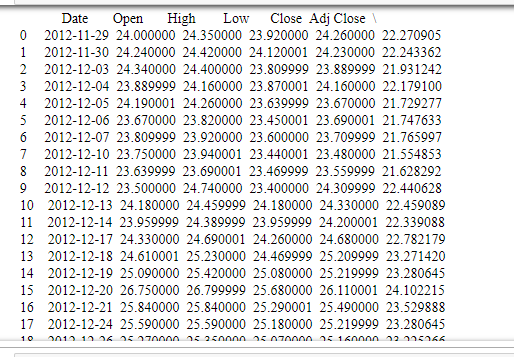
\includegraphics[width=0.5\textwidth]{datainputtest.png}
}
\caption{\label{Spark}}
\end{center}
\end{figure}
\end{enumerate}

\subsection{Plot Testing\\}

Type: Functional, Manual, Static
Initial State: NA\\
Input: A dataset file\\
Output: A correct plot\\
How test will be performed: System reads the data and generate a plot using the price and the date as the x and y axis.\\
result : Pass. The screen shot shows the result of the plot. It displays the historical data of four companies from 2013 to the end of 2017.\\

~\newline
\begin{figure}[h!]
\begin{center}
%\rotatebox{-90}
{
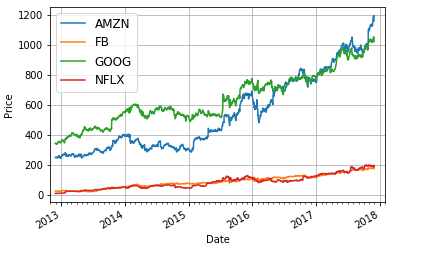
\includegraphics[width=0.5\textwidth]{plottest.png}
}
\caption{\label{plot}}
\end{center}
\end{figure}


~\newline

\subsection{Distributed System}
This section focus on the distributed system of Spark platform. It guides the
users to test the data flow on the spark system. RDD is the format of data flow
in Spark. testers need to double check the data was distributed into each
workers through RDD.

\paragraph{ Spark RDD Testing}
~\newline

%\begin{enumerate}

%\item{Data is distributed to workers\\}

Type: Functional, Manual, Static\\
Initial State: NA\\
Input: There will be a list of numbers to input to the RDD function. To test the RDD function, the driver will ask Spark to return some random number back. \\
Output: The list of numbers which is collected back from workers.\\
How test will be performed: There will be an input array to the driver, driver assign the array to each workers. Each worker receives part of the numbers in the list. When the driver collect the RDD, works return each part of the number back to driver. \\
Result: Pass. The screen shot shows the system assign an array of integers from 0 to 1000 and collect 5 samples back.
~\newline

\begin{figure}[h!]
\begin{center}
%\rotatebox{-90}
{
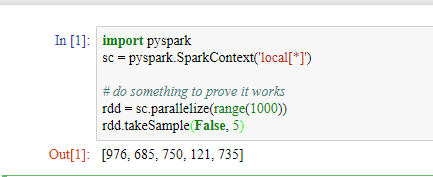
\includegraphics[width=0.5\textwidth]{sparktest.png}
}
\caption{\label{Spark}}
\end{center}
\end{figure}
~\newline


%\end{enumerate}


\section{Nonfunctional Requirements Evaluation}

\subsection{Usability}
This test needs to be done under a Spark environment. Docker container is suggested. 
Python and Spark are required to be installed in the container and the following frameworks are required for Python :\\ 
pandas, numpy, sklearn, matplotlib and pyspark\\

\begin{enumerate}
\item{Participants\\}
Classmate: Li Shusheng 
\item{Document given\\}
\url{https://github.com/renjiezhang/CAS-741/blob/master/src/Installation Instruction.pdf}
\item{Task for participants\\}
Read the Installation Instruction, install the necessary tools and frameworks and run the test successfully. 
\item{How test will be measured and performed\\}
If all participants can run test case successfully with the instruction, then Usability of the program is good.
\item{Result\\} Docker for windows does not work on windows home edition, it works on professional edition since it needs the Hyper-V feature to be turned on. Everything else works fine with a proper windows edition.
\end{enumerate}


\subsection{Performance}
Type: Manual\\
Initial State: NA\\
Input/Condition: NA\\
Output/Result: Result of the time cost\\
How test will be performed: \\
Chang the size of the dataset files by downloading the files with different date range. For example, reduce the date range from 5 years to 3 years and compare the performance. \\
Change the number of date parameter to predict short term and long term stock price. By adding a new type of number of date, the software need to increase the run time. \\
Result: The prediction accuracy was influenced by the days of the prediction. The longer term (90,270) is more accurate then the shorter term(1,5). \\ 
The performance of 5 years dataset file with 4 types of prediction dates is about 36 seconds. By reducing the prediction date types from 4 to 3, the execution time become to 21 seconds. \\
The performance result is on the result.txt
\section{Comparison to Existing Implementation} 

The test on multiple spark workers was not implemented but the source code has been changed to Spark based. I have encountered some problems with configuration of multiple Docker containers and I don't have enough time to solve the problem. The system for now is on a single node Spark worker.

\section{Unit Testing}

The unit testing plan will involve the following modules: Load Data, SVM Kernelling, Volatility Calculating, Momentum Calculating, Predict and Output.\\
\begin{enumerate}

\item{ Calculate Volatility\\}
This function is use to calculate the price volatility and index volatility. Since the calculation is similar they share the same function. A correct result is expected by inputting the parameters to the equation \\
$\frac{\sum_{i=t-n+1}^{t} \frac{C_i-C_{i-1}}{C{i-1}}}{n}$ \\ 

Input: A pre-defined Array of stock record, which contains two elements: price and date\\
Output: An array of price volatility based on the input array\\


\item{ Calculate Momentum\\}
This function is use to calculate the price momentum and index momentum. Since the calculation is similar they share the same function. A correct result is expected by inputting the parameters to the equation \\
$\frac{\sum_{i=t-n+1}^{t} \frac{C_i-C_{i-1}}{C{i-1}}}{n}$ \\ 

Input: A pre-defined Array of stock record, which contains two elements: price and date\\
Output: An array of price volatility based on the input array\\


\item{Predict \\}
The Predict module receives a set of parameters calculated from the previous functions and returns a result. A correct result is expected by inputting the parameters to the equation \\\\
$y=\beta _0+\sum {a_iy_iK(x(i),x)}$\\
Input: Two pre-defined lists of stock record, which contains two elements: price and date. They have same format, one is for stock price and another is for NASDQ Index record\\
Output:A score of a decimal number which represents the probability\\

The result of the unit test is shown as the screen shot:
~\newline
\begin{figure}[h!]
\begin{center}
%\rotatebox{-90}
{
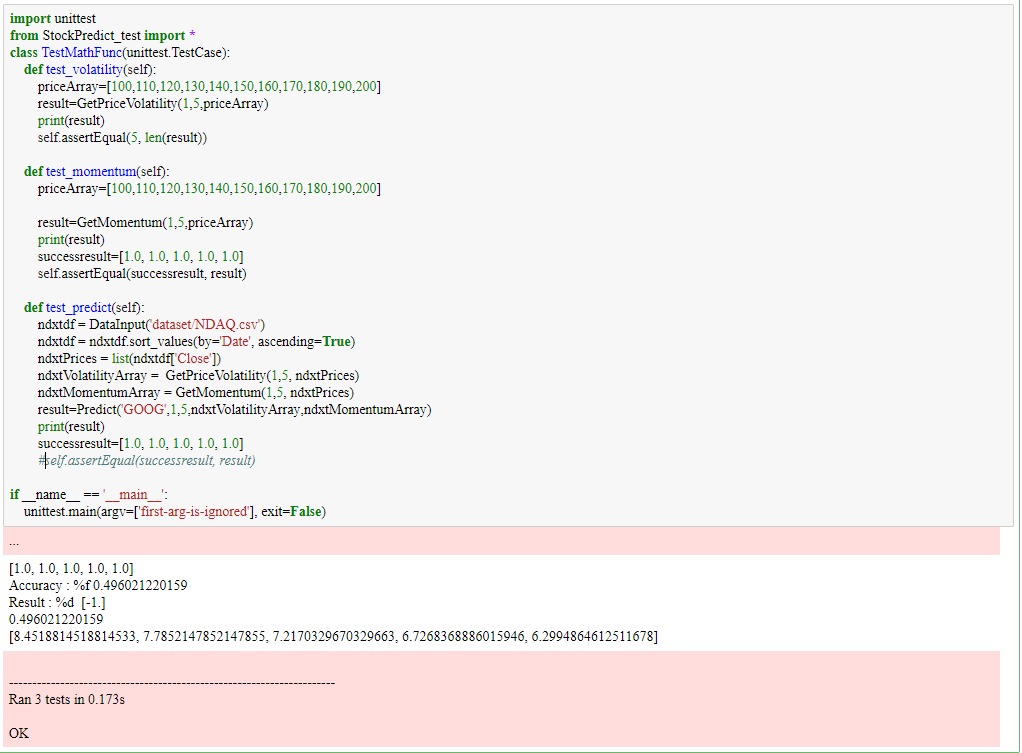
\includegraphics[width=0.5\textwidth]{unittest.png}
}
\caption{\label{Spark}}
\end{center}
\end{figure}
\end{enumerate} 

\section{Changes Due to Testing}
Since the kernelling function K is given by the library, the T2 of kernelling function is removed from SRS\\
Plot module was moved from software decision model to behavior-hiding module because the x ray has been customized to display by years not days. 

\section{Automated Testing}
NA
\section{Trace to Requirements}

\noindent \begin{itemize}

\item[R\refstepcounter{reqnum}\thereqnum \label{R_Inputs}:] Input data 

\item[R\refstepcounter{reqnum}\thereqnum \label{R_OutputInputs}:] Polt

\item[R\refstepcounter{reqnum}\thereqnum \label{R_Calculate}:] SVM Calculation

\item[R\refstepcounter{reqnum}\thereqnum \label{R_VerifyOutput}:] Verification

\item[R\refstepcounter{reqnum}\thereqnum \label{R_Output}:] Output
\end{itemize}

~\newline
\begin{table}[h!]
\centering
\begin{tabular}{|c|c|c|c|c|c|c|c|}
\hline
& \rref{R_Inputs}& \rref{R_OutputInputs} & \rref{R_Calculate}& \rref{R_VerifyOutput}& \rref{R_Output} \\
\hline


Input Test &x&x & &x &\\ \hline
Plot Test & &x & & & \\ \hline
Spark test && & & & \\ \hline
Volatility Test & & x& & &x \\ \hline
Momentum Test & & x& & &x \\ \hline
Predict Test & & x& & &x \\ \hline
\hline
\end{tabular}

\label{Table:R_trace}
\end{table}
\section{Trace to Modules} 
\begin{description}
\item [\refstepcounter{mnum} \mthemnum \label{mHH}:] Hardware-Hiding Module
\item [\refstepcounter{mnum} \mthemnum \label{mInput}:] Data Input Module
\item [\refstepcounter{mnum} \mthemnum \label{mKernelling}:]Kernelling Module
\item [\refstepcounter{mnum} \mthemnum \label{mVolatility}:] Price Volatility Module
\item [\refstepcounter{mnum} \mthemnum \label{mMomentum}:] Price Momentum Module
\item [\refstepcounter{mnum} \mthemnum \label{mPrediction}:] Stock Prediction Module
\item [\refstepcounter{mnum} \mthemnum \label{mOutput}:] Output Module
\item [\refstepcounter{mnum} \mthemnum \label{mSpark}:] Spark RDD Module
\item [\refstepcounter{mnum} \mthemnum \label{mPlot}:] Data Plot Module
\end{description}

\begin{table}[h!]
\centering
\begin{tabular}{|c|c|c|c|c|c|c|c|c|c|}
\hline
& \mref{mHH}& \mref{mInput}& \mref{mKernelling}& \mref{mVolatility}& \mref{mMomentum}& \mref{mPrediction}& \mref{mOutput}& \mref{mSpark}& \mref{mPlot}\\
\hline
Input Test &&x&& && & & &x\\ \hline
Plot Test &&&& & & & & &x \\ \hline
Spark test &&&& && & & x& \\ \hline
Volatility Test &&&& x& & & & & \\ \hline
Momentum Test &&&& &x & & & & \\ \hline
Predict Test &&&& x& x&x & x& & \\ \hline

\end{tabular}
\label{Table:R_trace}
\end{table}
\section{Code Coverage Metrics}
NA
\bibliographystyle{plainnat}

\bibliography{SRS}

\end{document}

